\section{Experiments}

\begin{table}
	\centering
	\begin{tabular}{|c||c|c|c|c|} \hline
		Data split & Source & Segmented & Images & Patients \\\hline
		Training & \vtop{\hbox{\strut Med-Seg}\hbox{\strut ICTCF}}&
		\vtop{\hbox{\strut Yes}\hbox{\strut No}} & 
		\vtop{\hbox{\strut 699}\hbox{\strut 6654}}&
		\vtop{\hbox{\strut 39}\hbox{\strut 1338}}\\\hline
		Validation & Med-Seg & Yes & 115 & 35 \\\hline
		Testing & Med-Seg & Yes & 118 & 35 \\\hline
	\end{tabular}
	\caption{This table shows the data distribution between the datasets that we use to evaluate our model on. Med-Seg refers to the COVID-19 CT Segmentation data set and ICTCF refers to the ICTCF data set.}
	\label{tab:dataset}
\end{table}

\begin{table*}
	\centering
	\begin{tabular}{| c | c || c c c c c ||}
	\hline
	Methods & & Dice & Jaccard & Sen. & Spec. & MAE \\ \hline
	Single SInfNet &  Mean & 0.66 & 0.65 & 0.45 & 0.99 & 14.43 \\ \cline{2-7}
						   & Error & $\pm$ 0.06 & $\pm$ 0.05 & $\pm$ 0.07 & $\pm$ 0.00 & $\pm$ 0.77 \\ \hline
	Single SInfNet + data aug(0.4) &  Mean & 0.61 & 0.62 & 0.38 & 0.99 & 16.31 \\ \cline{2-7}
	& Error & $\pm$ 0.06 & $\pm$0.05 &$\pm$0.07 &$\pm$0.00 &$\pm$0.90 \\ \hline
	Single SInfNet + data aug (0.5) &  Mean &0.64 &0.63 &0.41 &0.99 & 14.67 \\ \cline{2-7}
	& Error &$\pm$0.06 &$\pm$0.05 &0.07 &$\pm$0.00 & $\pm$0.82 \\ \hline \hline
	Single Self-SInfNet &  Mean & & & & & \\ \cline{2-7}
	& Error & & & & & \\ \hline
	Single Self-SInfNet + data aug &  Mean & & & & & \\ \cline{2-7}
	& Error & & & & & \\ \hline
	\end{tabular}
	\caption{Quantitative result for comparison between Single segmentation InfNet and self-supervised single segmentation InfNet}
	\label{tab:single}
\end{table*}

\begin{table*}
	\centering
	\begin{tabular}{| c | c || c c c c c || c c c c c |}
		\hline
		& &\multicolumn{5}{c||}{Ground-Glass Opacity} & \multicolumn{5}{c|}{Consolidation}\\ \cline{3-12}
		Methods & & Dice & Jaccard & Sen. & Spec. & MAE & Dice & Jaccard & Sen. & Spec. & MAE \\\hline
		Multi SInfNet & Mean & 0.32 & 0.43 & 0.40 & 0.993 & 0.32 & 0.18 & 0.45  & 0.20 & 0.996 & 0.007  \\ \cline{2-12}
		& Error & 0.004 & 0.05 & 0.06 & 0.003 & 0.004 & 0.05 & 0.04 & 0.06 & 0.001 & 0.003 \\ \hline \hline
		
		Multi SInfNet + data aug(0.4) & Mean & 0.28 & 0.37 & 0.35 & 0.993 & 0.01 & 0.14 & 0.38 & 0.16 & 0.994 & 0.01  \\ \cline{2-12}
		& Error & 0.05 & 0.03 & 0.06 & 0.003 & 0.004 & 0.04 & 0.04 & 0.05 & 0.002 & 0.004  \\ \hline \hline
		
		Multi SInfNet + data aug(0.5) & Mean & 0.30 & 0.42 & 0.37 & 0.993 & 0.01 & 0.15 & 0.45 & 0.15 & 0.997 & 0.007  \\ \cline{2-12}
		& Error & 0.05 & 0.03 & 0.06 & 0.003 & 0.004 & 0.05 & 0.03 & 0.05 & 0.001 & 0.004  \\ \hline \hline
		
		Multi Self-SInfNet & Mean & & & & & & & & & &  \\ \cline{2-12}
		& Error & & & & & & & & & &  \\ \hline \hline
		
		Multi Self-SInfNet + data aug & Mean & & & & & & & & & &  \\ \cline{2-12}
		& Error & & & & & & & & & &  \\ \hline \hline
	\end{tabular}
	\caption{Quantitative result of Ground-glass Opacities \& Consolidation on the test data set. Prior is obtained from the single segmentation InfNet}
\end{table*}

\begin{table*}
	\centering
	\begin{tabular}{| c | c || c c c c c || c c c c c |}
		\hline
		& &\multicolumn{5}{c||}{Ground-Glass Opacity} & \multicolumn{5}{c|}{Consolidation}\\ \cline{3-12}
		Methods & & Dice & Jaccard & Sen. & Spec. & MAE & Dice & Jaccard & Sen. & Spec. & MAE \\\hline
		Multi SInfNet & Mean & 0.55 & 0.72 & 0.60 & 0.996 & 0.005 & 0.21 & 0.57  &0.23  &0.998  &0.004   \\ \cline{2-12}
		& Error & 0.07 & 0.03 & 0.08 & 0.003 & 0.003 & 0.06 & 0.03 & 0.07 & 0.0007 & 0.002 \\ \hline \hline
		
		Multi SInfNet + data aug(0.4) & Mean &  &  &  &  &  &  &  &  &  &   \\ \cline{2-12}
		& Error &  &  &  &  &  &  &  &  &  &   \\ \hline \hline
		
		Multi SInfNet + data aug(0.5) & Mean &  &  &  &  &  &  &  &  &  &   \\ \cline{2-12}
		& Error &  &  &  &  &  &  &  &  &  &   \\ \hline \hline
		
		Multi Self-SInfNet & Mean & & & & & & & & & &  \\ \cline{2-12}
		& Error & & & & & & & & & &  \\ \hline \hline
		
		Multi Self-SInfNet + data aug & Mean & & & & & & & & & &  \\ \cline{2-12}
		& Error & & & & & & & & & &  \\ \hline \hline
	\end{tabular}
	\caption{Quantitative result of Ground-glass Opacities \& Consolidation on the test data set. Prior is obtained from the test set.}
\end{table*}

\iffalse
\begin{table*}
	\centering
	\begin{tabular}{|c|c|c|c|c|} \hline
		& Dice & Jaccard & Sensitivity & Specificity \\\hline
		single SInfNet &  &  &  &  \\\hline
		single SInfNet + data aug(0.4) &  &  &  &  \\\hline
		single SInfNet + data aug(0.5) &  &  & &  \\\hline \hline
		single Self-super & & & & \\\hline
		single Self-super+data aug & & & & \\\hline \hline
		multi SInfNet & & & & \\\hline
		multi SInfNet + data aug(0.4) & & & & \\\hline
		multi SInfNet + data aug(0.5) & & & & \\\hline \hline
		multi Self-super & & & & \\\hline
		multi Self-super+data aug & & & & \\\hline \hline
		
	\end{tabular}
	\caption{Comparison of supervised inf-net (SInf-Net) model with added data augmentation.  The floating value  after the data augmentation refers to the fraction of the image randomly cutout. 0.2 shows that 0.2 of the image is cutout to be empty. The evaluation are done on the test set. }
\end{table*}
\fi


\subsection{Datasets}
The dataset that we will be using is an integrative resource of chest computed tomography images and clinical features of patients with COVID-19 pneumonia (ICTCF) \cite{ref23} which contains the severity score for each CT lung image and CT lung images from medical segmentation website \cite{ref26}. 

ICTCF contains 127 types of clinical features and laboratory confirmed cases of COVID-19 from 1170 patients including the severity for the CT lung images. However, ICTCF dataset does not contain the segmentation labels for the ground-glass opacities and the consolidation in the CT lung images. In total, there are 6654 of CT lung images in ICTCF dataset. Originally, there were 1521 patients. However, some of the patients are missing CT lung images. We remove these patients that are missing CT lung images. After preprocessing the patients, the dataset was left with 1338 patients that contains CT lung images. The dataset can be found here: http://ictcf.biocuckoo.cn/. 

As for the medical segmentation dataset, they contain ground truth label for the segmentation for ground-glass opacities and consolidation of the CT lung images but does not contain the severity score for the CT Lung images. The total amount of CT lung images contain in medical segmentation dataset is 932 CT lung images. We randomly assign the CT lung images into training set, validation set, and testing set of which the training set contains 699 CT lung images, the validation set contains 115 CT lung images, and the testing set contains 118 CT lung images. 

The assignment of the dataset can be seen in \ref{tab:dataset}.


\begin{figure}
	\centering
	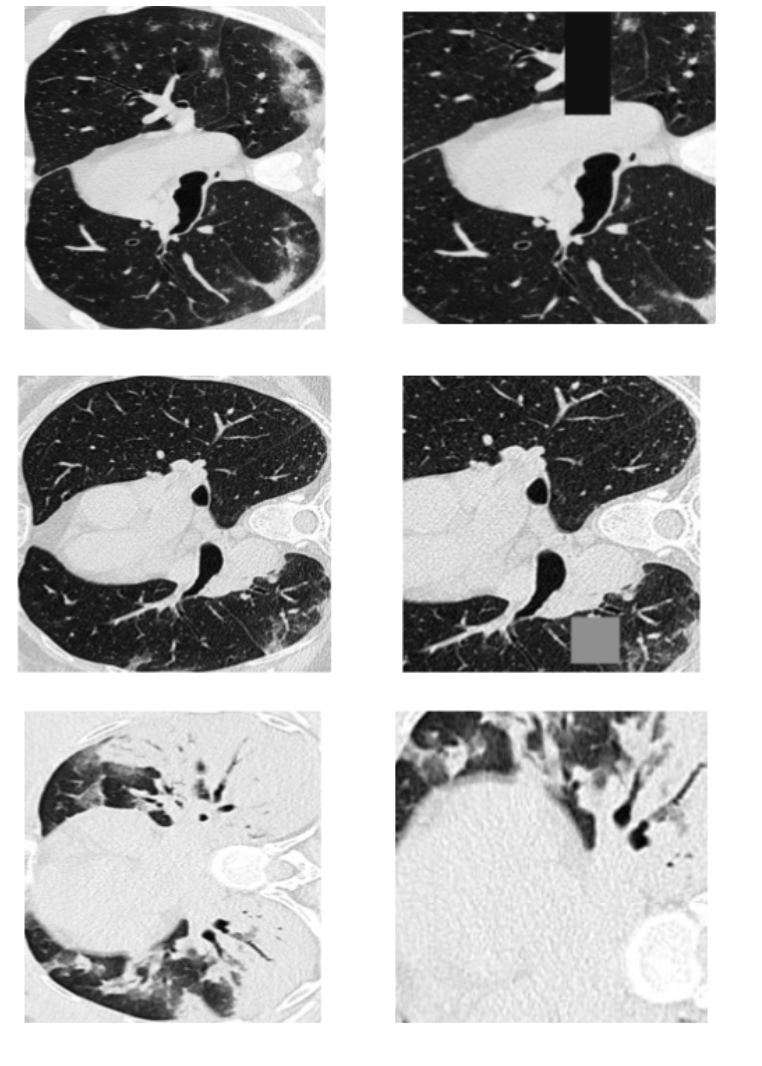
\includegraphics[width=\linewidth]{data_aug.png}
	\caption{Example CT lung images of our data augmentation. The left column is the original CT lung images while the right column is the augmented CT lung images. The first row of the CT lung images involves random cropping and random cutout. The second row of the CT lung images involves random cropping and random cutout. The third row of the CT lung images involves random cropping and vertical flipping. We can see the random cutout involves patching the image with colors of the same value of rgb. For instance, if the value of r is 10, then the value of g and b are also 10. If the value of r is 50, then the value of g and b are also 50.}
	\label{fig:data_aug}
\end{figure}

\subsection{Data Augmentation}
We used data augmentation to increase our data samples size. The data agumentation that we used includes \textit{vertical flipping, horizontal flipping, random crop, and random cutout}. For the random cutout percentage, we experimented that 0.5 cutout of the CT lung images yield higher performance than the rest of the value. This is because entropy at 0.5 is the highest which could increase more variability of the images. Examples of the data augmentation can be seen in figure \ref{fig:data_aug}.

